\chapter{Compositions}
\label{appendix:dos}

\section{Projected density of states}

\begin{figure}[H]
	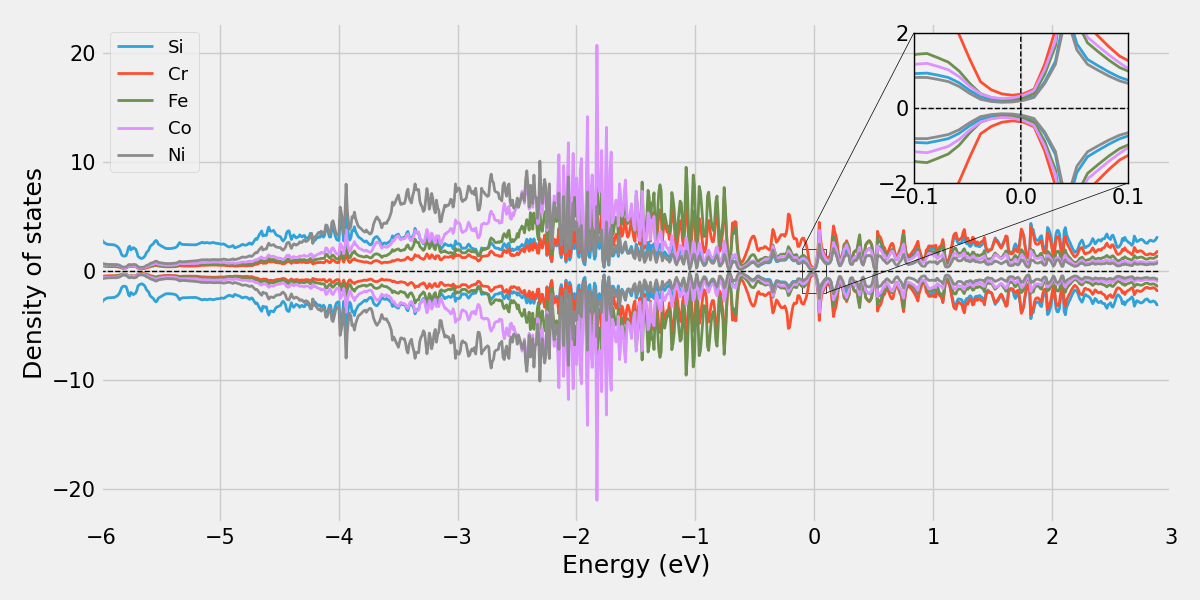
\includegraphics[width=\textwidth]{results/fesi2/composistions/crfeconi_PDOS.png}
	\caption{ch{Cr4Fe4Co4Ni4Si32}}
\end{figure}

\begin{figure}[H]
	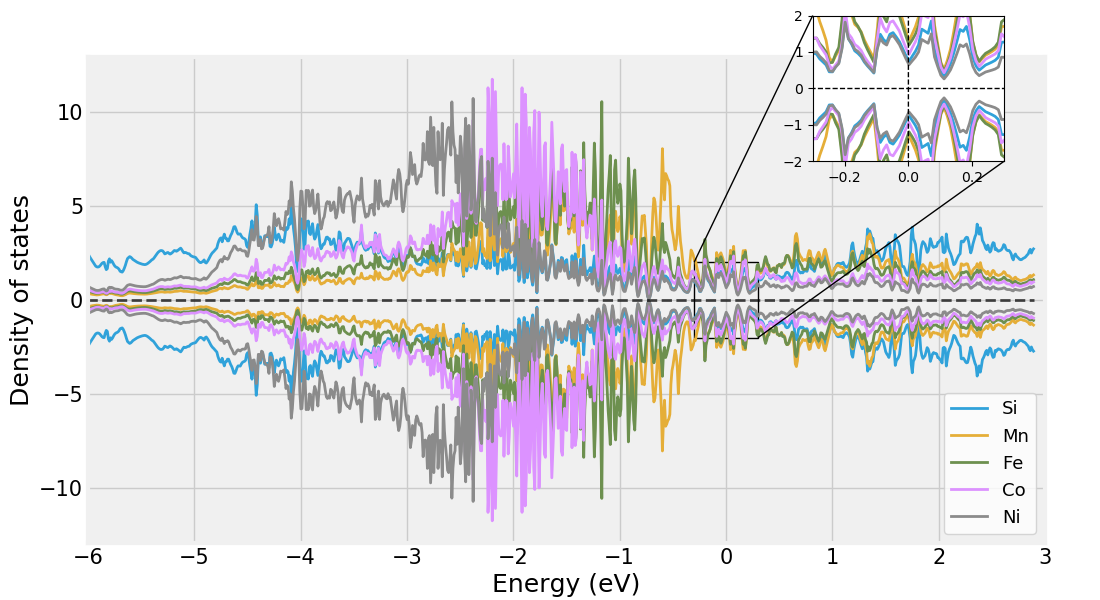
\includegraphics[width=\textwidth]{results/fesi2/composistions/cofemnni_PDOS.png}
	\caption{ch{Co4Fe4Mn4Ni4Si32}}
\end{figure}

\begin{figure}[H]
	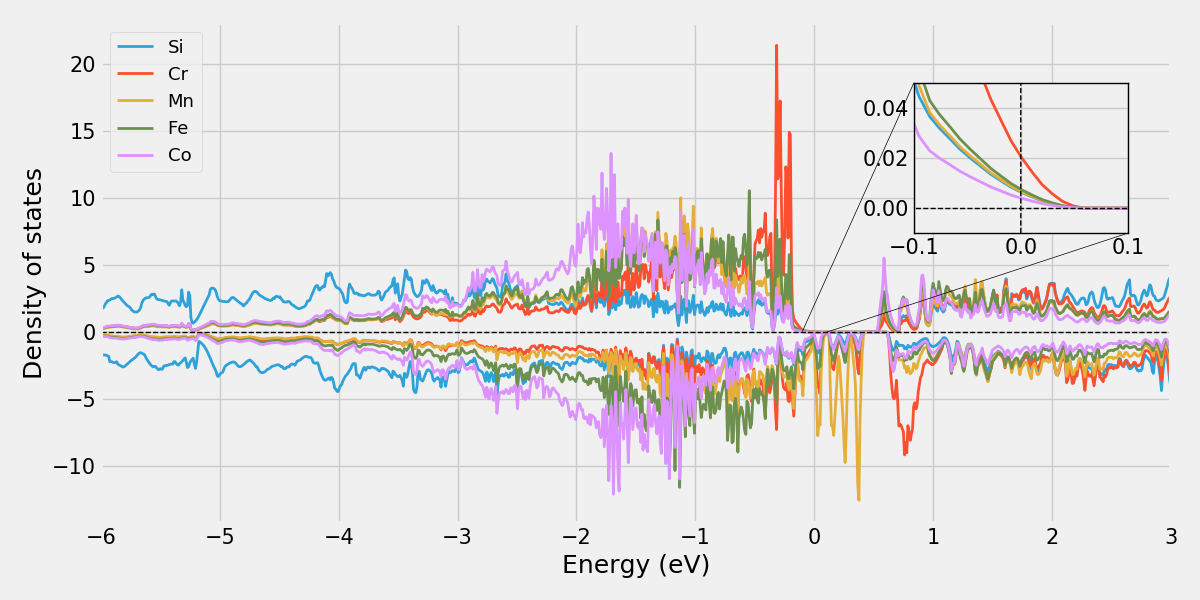
\includegraphics[width=\textwidth]{results/fesi2/composistions/crfemnco_PDOS.png}
	\caption{ch{Cr4Fe4Mn4Co4Si32}}

\end{figure}

\begin{figure}[H]
	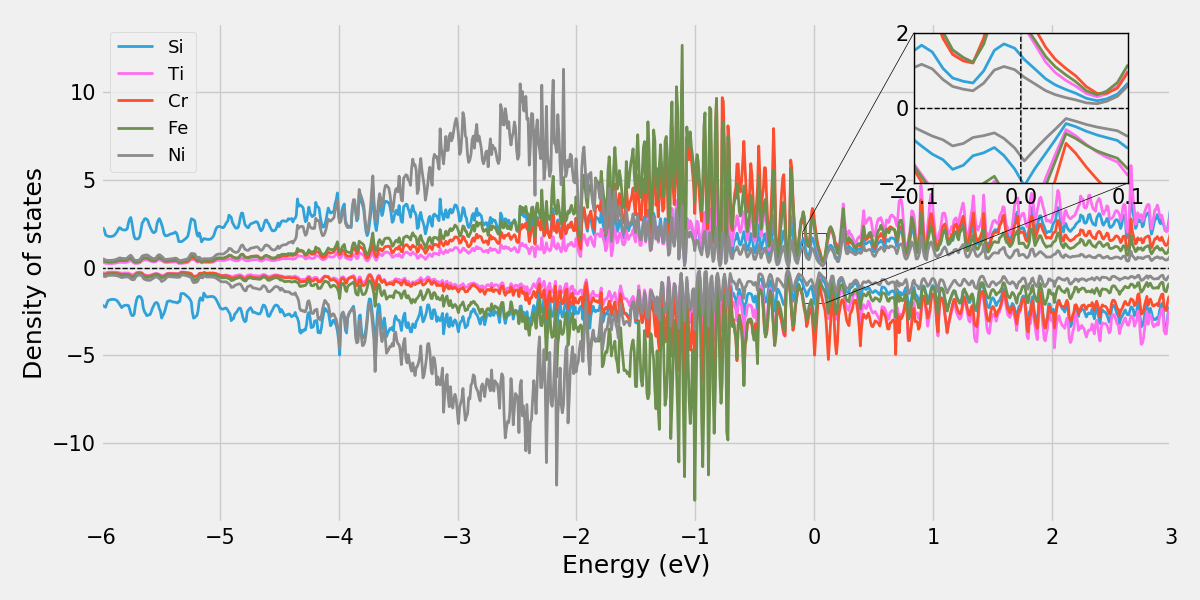
\includegraphics[width=\textwidth]{results/fesi2/composistions/crfetini_PDOS.png}
	\caption{ch{Cr4Fe4Ti4Ni4Si32}}

\end{figure}

\begin{figure}[H]
	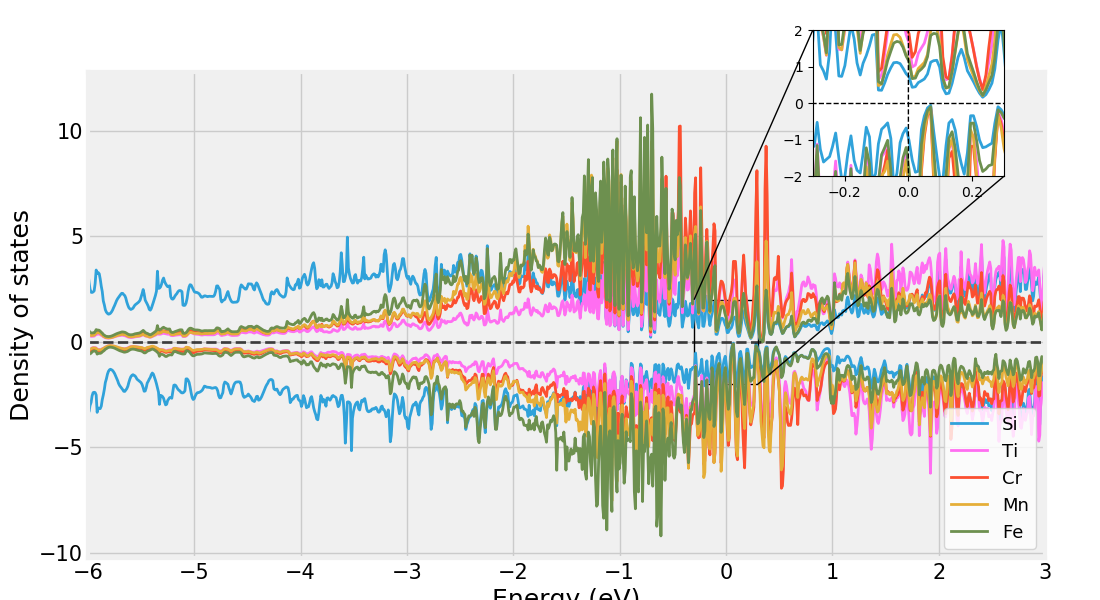
\includegraphics[width=\textwidth]{results/fesi2/composistions/crfemnti_PDOS.png}
	\caption{ch{Cr4Fe4Mn4Ti4Si32}}
\end{figure}

\section{Probability distribution functions}

\begin{figure}[H]
	\centering
	\begin{subfigure}{\textwidth}
		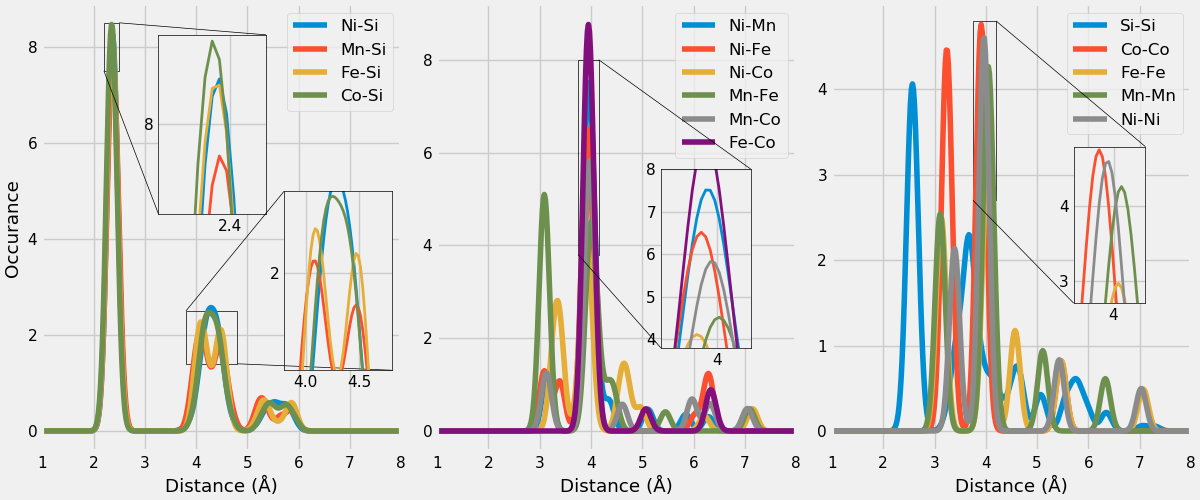
\includegraphics[width=\textwidth]{results/fesi2/composistions/cofemnni_PDF.png}
	\end{subfigure}
	\begin{subfigure}{\textwidth}
		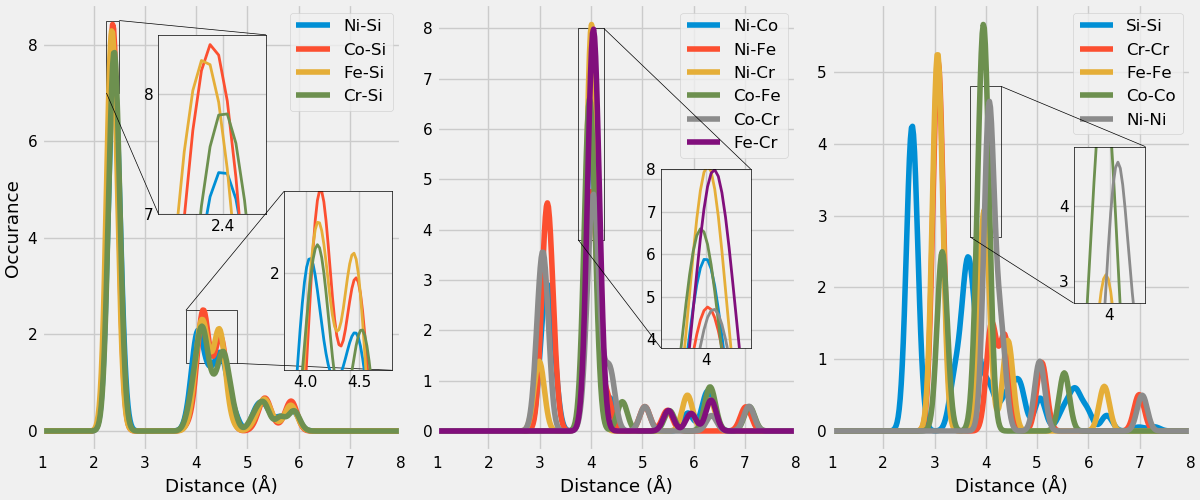
\includegraphics[width=\textwidth]{results/fesi2/composistions/crfeconi_PDF.png}
	\end{subfigure}
	\begin{subfigure}{\textwidth}
		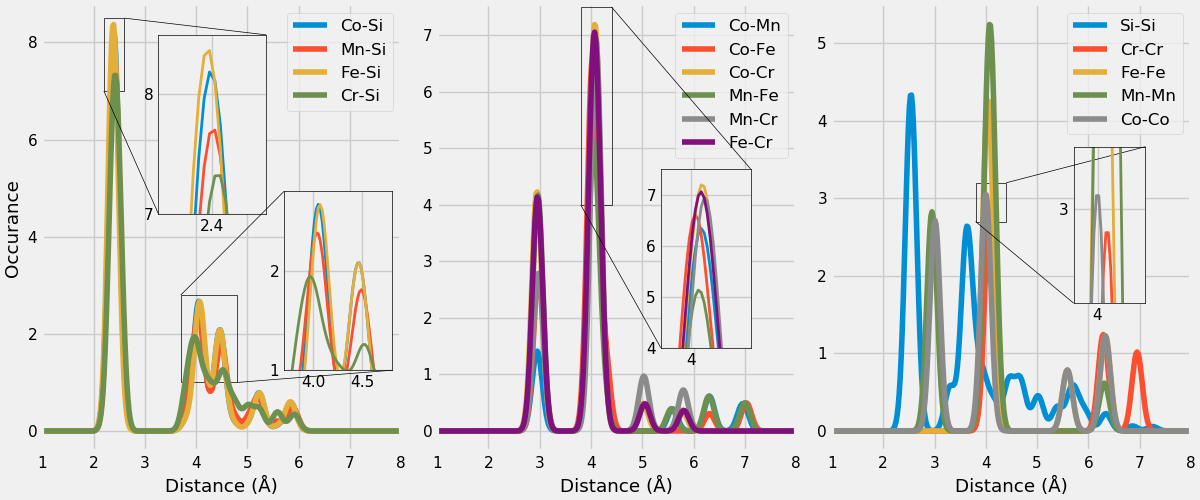
\includegraphics[width=\textwidth]{results/fesi2/composistions/crfemnco_PDF.png}
	\end{subfigure}
	\caption{Probability distribution functions of top: \ch{Co4Fe4Mn4Ni4Si32} (SQS D), middle: \ch{Cr4Fe4Co4Ni4Si32} (SQS B), bottom: \ch{Cr4Fe4Mn4Co4Si32} (SQS B)}
\end{figure}
Similarly we look at the PDFs of \ch{Cr4Fe4Mn4Ti4Si32} and \ch{Cr4Fe4Ti4Ni4Si32} bellow.
\begin{figure}[H]
	\centering
	\begin{subfigure}{\textwidth}
		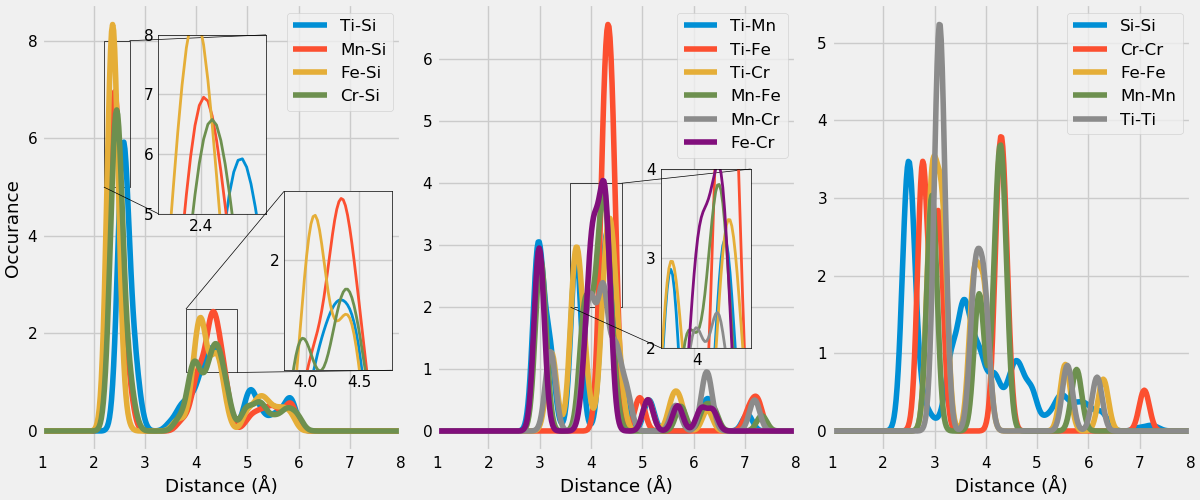
\includegraphics[width=\textwidth]{results/fesi2/composistions/crfemnti_PDF.png}
	\end{subfigure}
	\begin{subfigure}{\textwidth}
		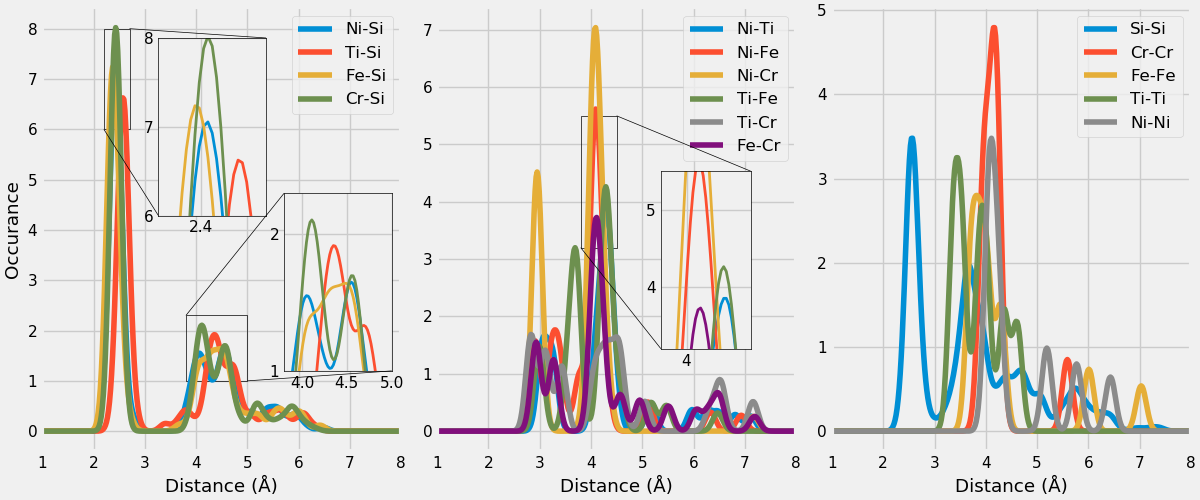
\includegraphics[width=\textwidth]{results/fesi2/composistions/crfetini_PDF.png}
	\end{subfigure}
	\caption{Probability distribution function of top: \ch{Cr4Fe4Mn4Ti4Si32} (SQS B), bottom: \ch{Cr4Fe4Ti4Ni4Si32} (SQS B))}
\end{figure}